\documentclass[a5paper,11pt,openany]{article}

\usepackage{orcidlink}

\usepackage[top=2cm,bottom=2cm,bindingoffset=0cm]{geometry}

\usepackage[svgnames]{xcolor} % Required to specify font color

%\documentclass[a4paper,12pt,openany]{scrbook}

%\usepackage{glossaries}
%\usepackage[xindy]{glossaries}
%\makeglossaries

%\usepackage{odsfile,lmodern}

%\usepackage{luacode}

\usepackage{multicol}

%\usepackage{churchslavonic}
%\usepackage{polyglossia}
%\setotherlanguages{russian,churchslavonic}

\usepackage{mathtext}
\usepackage{makeidx}
%\usepackage{imakeidx}
\usepackage{longtable}
\usepackage[tc]{titlepic}

\usepackage{fontspec}

\usepackage[protrusion=true,expansion,
tracking=true,letterspace=50]{microtype}

%\SetTracking[ spacing = {25*,166, } ]{ encoding = *, shape = sc }{ 25 }


%\usepackage{soulutf8}
%\usepackage{letterspace}

%\usepackage[toc]{appendix}
\usepackage[toc,titletoc]{appendix}
\renewcommand\appendixtocname{Appendix}
\renewcommand\appendixpagename{Appendix}

%\usepackage{xunicode}
\usepackage{xltxtra}

\usepackage[normalem]{ulem}
\usepackage{adjustbox}

\usepackage{polyglossia}
\setmainlanguage{english}
\setdefaultlanguage{english}
\setotherlanguage{russian}
\setotherlanguage{english}
\setotherlanguage{greek}
\setotherlanguage{latin}
\setotherlanguage{polish}


\setmainfont[BoldFont={DejaVuSerif-Bold.ttf},
ItalicFont={DejaVuSerif-Italic.ttf},
 BoldItalicFont={DejaVuSerif-BoldItalic.ttf}]{DejaVuSerif.ttf}

\setromanfont[BoldFont={DejaVuSerif-Bold.ttf},
ItalicFont={DejaVuSerif-Italic.ttf},
 BoldItalicFont={DejaVuSerif-BoldItalic.ttf}]{DejaVuSerif.ttf}

\setsansfont[BoldFont={DejaVuSans-Bold.ttf},
ItalicFont={DejaVuSans-Oblique.ttf},
 BoldItalicFont={DejaVuSans-Oblique.ttf}]
{DejaVuSans.ttf}

\setmonofont[BoldFont={DejaVuSansMono-Bold.ttf},
ItalicFont={DejaVuSansMono-Oblique.ttf},
 BoldItalicFont={DejaVuSansMono-BoldOblique.ttf}]
{DejaVuSansMono.ttf}



\usepackage{enumitem}
\usepackage{indentfirst} 

\usepackage{verse}

\usepackage{graphicx}

%\usepackage[pdfpagelabels,unicode,plainpages=false]{hyperref}

\hypersetup{pdftitle=How Prince Vladimir Overthrew the Idols. Петр Семилетов.}

\usepackage{bookmark} 
\usepackage{relsize}

\usepackage{tocloft,calc}
\usepackage[nottoc,numbib]{tocbibind}

\frenchspacing
\righthyphenmin=2

\makeatletter
\@addtoreset{chapter}{part}
\makeatother  


%\titlepic{\includegraphics[width=0.50\textwidth]{cover/04.jpg}}

\title{HOW VLADIMIR THE GREAT\\OVERTHREW THE IDOLS\\
\textsmaller[2]{edition 1.0}}
\author{Peter Semiletov\\ORCID:0009-0002-3901-7785 \orcidlink{0009-0002-3901-7785}}
\date{24/11/2024}




\newcommand*{\plogo}{\fbox{$\mathcal{PL}$}} % Generic publisher logo

% –  –  –  –  –  –  –  –  –  –  –  –  –  –  –  –  –  –  –  –  –  –  –  –  –  –  –  –  –  –  –  –  –  –  –  –  –  –  –  –  –  –  –  – 
%	TITLE PAGE
% –  –  –  –  –  –  –  –  –  –  –  –  –  –  –  –  –  –  –  –  –  –  –  –  –  –  –  –  –  –  –  –  –  –  –  –  –  –  –  –  –  –  –  – 

\newcommand*{\titleAT}{\begingroup % Create the command for including the title page in the document
\newlength{\drop} % Command for generating a specific amount of whitespace
\drop=0.1\textheight % Define the command as 10% of the total text height

\rule{\textwidth}{1pt}\par % Thick horizontal line
\vspace{2pt}\vspace{-\baselineskip} % Whitespace between lines
\rule{\textwidth}{0.4pt}\par % Thin horizontal line

\vspace{\drop} % Whitespace between the top lines and title
\centering
\textcolor{Red}{
{\Huge HOW VLADIMIR THE GREAT\\ OVERTHREW THE IDOLS}\\[0.5\baselineskip] % Title line 1
%{\Large}\mbox{}\\[0.75\baselineskip] % Title line 2
%{\Huge четвертая редакция}} % Title line 3
}

\vspace{0.25\drop} 
\rule{0.3\textwidth}{0.4pt}\par 

\mbox{ }\\
редакция 1.0\\

%\includegraphics[width=0.40\textwidth]{cover/04.jpg}

\vspace{\drop} 

{\Large \textsc{Peter Semiletov\\https://psemiletov.github.io}}\par 


\vfill
%{\large \textcolor{Red}{\plogo}}\\[0.5\baselineskip] % Publisher logo
{\large \textsc{2024}}\par % Publisher

\vspace*{\drop} 

\rule{\textwidth}{0.4pt}\par
\vspace{2pt}\vspace{-\baselineskip} 

\rule{\textwidth}{1pt}\par 

\endgroup}


\begin{document}

\pagestyle{empty}

\maketitle

\newpage

\pagestyle{plain}

%\tableofcontents

%\input{pre/pre.tex}
%\input{plan-right/plan-right.tex}
%\input{plan-right/plan-right-text.tex}

%\begin{abstract}
%The Baptism of Rus by Prince Vladimir the Red Sun – was it truly a step toward a new faith, or is there more to it? Why did Vladimir deem it necessary to publicly overthrow the idols in the presence of Christian priests invited from Chersonesus, and why did this act not provoke outrage among the people against the prince?
%\end{abstract}

\begin{abstract}
The famous baptism of Rus' in Kiev by Prince Vladimir the Great—a course towards a new faith, or is there some trickery in this? Why did Vladimir need the public overthrow of idols in the presence of Christian priests invited from Chersonesus, and why did this overthrow not provoke the people's outrage against the prince? Judging by everything, the prince performed a pagan ritual in the process.
\end{abstract}


\section{How Vladimir Overthrew the Idols}

I will greatly simplify the narrative here, avoiding references to foreign sources about Vladimir, including Icelandic sagas, where the events surrounding the prince's life and the baptism of both Vladimir himself and Rus are described differently from Slavic sources.

In other words, the chronicles contain details absent in the sagas, while the sagas include aspects missing from the chronicles and hagiographies. If one were to overlay the information from the sagas onto the chronicles, it would appear that the baptism occurred twice—once according to Eastern rites and once according to Western rites—at different times and under different circumstances.

I intend to examine the Baptism of Rus precisely as it is described in \textit{Primary Chronicle}\cite{ipat} and several other ancient Slavic sources, such as the \textit{Kiev Synopsis}\cite{sinopsis} edited by Innokentiy Gizel and Sofonovych's \textit{Khroinica}\cite{sofonovich01}. These are sources that form the foundation of the commonly accepted history or are closely aligned with it.

If we evaluate the events leading up to the Baptism of Rus, it appears to be a geopolitical masterstroke. Let me remind you of what transpired, according to the official chronology and the primary versions of the chronicles.

In 985, Vladimir waged war against the Bulgars. Exactly which Bulgars remains unclear, as there were the Volga Bulgars—whose name, incidentally, derives from river's name, if you replace the "B" with a "V". Meanwhile, the Bulgars who migrated from the Volga to the Danube were also called Bulgars, and their descendants established the country now known as Bulgaria.

Researchers, as usual, drew the most illogical conclusion, and it is now generally accepted that Vladimir campaigned against the Volga Bulgars. However, the chronicle provides a specific detail about Vladimir’s route\footnote{Here and further, I cite \textit{Primary Chronicle} from the Ipatiev Codex, converting Old Slavonic letters into their modern equivalents for ease of reading and typesetting.}:

\begin{quotation}
\noindent Иде Володимир на Болгары с
Добрынею оуем своим в лодьях а Торкы берегом приведе на конех
\end{quotation}

Thus, Vladimir set out from Kiev with his army (his uncle, Dobrynya, was with him) in lodyas (boats)\footnote{Лодья, the vessel similar to the viking boat.}, while their allies, the Torks, traveled along the shore on horseback.

If you look at a map, you'll see that this route would allow one to travel along the Dnieper River to the Black Sea, and from there, reach Bulgaria. However, reaching the Volga Bulgaria by boat is quite difficult!

Vladimir's army defeats the Bulgars, but Dobrynya advises him not to make them vassals, suggesting that the Bulgars are strong and live in wealth:

\begin{quotation}
\noindent суть вси в сапозех, сим дани нам не платити, поидев искать лапотник
\end{quotation}. 

In other words, Dobrynya suggests they should go after the weaker people, the "lapotniks" (a term referring to peasants or common folk). Vladimir makes peace with the Bulgars and returns to Kiev.

A year later, in 986, according to the Chronicle, the Bulgars arrive in Kiev and offer Vladimir to adopt their faith. They are, as the chronicle notes, "Bokhmichi"—that is, Muslims. They explain the tenets of their religion, but Vladimir refuses, as he dislikes two aspects. The first is circumcision, and the second is the prohibition of alcoholic drinks. "No drink no fun for Rus," Vladimir replies humorously.

The entire chronicle entry for the year 986 is devoted to how representatives of various churches and religions come to Vladimir with proposals to adopt their faith. "Germans from Rome" arrive. Jews come. Finally, from the Greeks—that is, from Byzantium, the Greek branch of the Roman Empire—a philosopher arrives. He reports the most unappealing details about the other religions and asserts the truth of the Eastern Christian Church, while also recounting the Bible.

This chapter seems to have been artificially inserted into the narrative of the chronicle, although it is possible that, in reality, there was indeed an embassy sent to Vladimir by various religious groups with the aim of protecting the states where these structures held sway from the growing power of Kievan Rus.

However, I would remind you that just six years earlier, when Vladimir first began to rule in Kiev, he placed idols of the pantheon of pagan gods:

\begin{quotation}
\noindent постави кумиры на холму вне двора теремнаго . Перуна деревяна а голова его серебряна а оус золот и Хорса . и Дажьбога . и Стрибога . и Семарьгла. и Мокошь . и жряху им . наричуще богы и привожаху сыны своя и жряху бесом и оскверняху землю требами своими
\end{quotation}

Not only did he set up idols of Perun, Khors, Dazhbog, Stribog, Semargl, Mokosh, and call them gods, but he also brought his sons there and made offerings to \textit{besy} (demons). This is specifically mentioned, as the Chronicler then writes, "but the most merciful God does not wish the death of sinners." Why would Nestor the chronicler write this unless it implied the sacrifice of sons, especially considering the numerous concubines Vladimir had?

In 980, Vladimir places idols, and by 986, he is offered the opportunity to join one of the Abrahamic religions.

A year later, in 987, Vladimir sends his \textit{boyars} to investigate the offered faiths. The boyars travel to the Bulgars, then to the Germans, and finally to the Greeks. Upon returning, the boyars are inclined to think that the Greeks have the best faith, and they note that Princess Olga, who was wiser than all, adopted Christianity of the \textbf{Greek} rite. Vladimir then asks the boyars:

 "Where shall we accept baptism?"

 "Wherever you like," replied the boyars.

A year passes, and in 988, Vladimir marches with his army to the Byzantine city of Chersonesus. Today, Chersonesus is the ruins located near Sevastopol. Chersonesus belonged to the Eastern Roman Empire, referred to in the chronicle as the Greeks, now known as Byzantium. It was one of the centers of Christianity and trade.

And so, Vladimir unsuccessfully lays siege to the city, standing before its walls. However, among the inhabitants of Chersonesus, there was a traitor—a man named Anastas. He sent an arrow with a note to the enemy camp, to Vladimir:

\begin{quotation}
\noindent кладези яже суть за тобой от востока ис того вода идет по трубе копавше преимете воду
\end{quotation}

That is, the water from the well flows eastward through a pipe. Dig it up and shut off the water.

Vladimir, upon learning of this, as the chronicle writes:

\begin{quotation}
\noindent взрев на небо и рече: аще ся сбудеть, се имам креститися
\end{quotation}

He gazed up at the sky and said, "If it works out, we will be baptized!"

Next, Vladimir begins to blackmail the emperors Basil and Constantine to secure his baptism. In this light, the Chronicle's section about Vladimir choosing the Eastern rite of Christianity among other faiths seems strange. After all, if they were offering it willingly, why would he resort to force?

Whatever the case, Vladimir orders the pipe to be dug up and blocked. A great thirst begins in Chersonesus, and the city surrenders.

Vladimir, along with his \textit{drujina} (warriors), enters Chersonesus and sends a message to Constantinople (modern-day Istanbul). He essentially says, "I have taken Chersonesus. Do you want the same fate for your capital, Constantinople? If not, here are my terms. I have heard that you have a sister—give her to me in marriage. Then nothing will happen to your Constantinople."

The emperors, upon receiving this message, were dismayed and replied, "It is possible, but you are a pagan. First, be baptized, and you will become one of our fellow believers."

Vladimir sends a reply through his envoys, stating that he had already learned about their faith and worship and that he finds it good.

The sister of Basil and Constantine, Anna, did not want to marry Vladimir, but her brothers told her that through this union, God would bring the land of Rus to repentance and save the Byzantine land from a fierce army. And so, they sent Anna to Chersonesus, accompanied by nobles and \textit{presbyters} (priests).

At that time, while in Chersonesus, Vladimir "fell ill in his eyes" and could see nothing. He sat in sorrow, unsure of what to do. Anna advised him to be baptized quickly to be healed and regain his sight. Then priests from Constantinople, along with local priests from Chersonesus, baptized Vladimir in the Church of St. Sophia. He immediately regained his sight. Witnessing this miracle, Vladimir and some of his warriors were baptized. After his baptism, Vladimir was betrothed to Anna.

The Chronicler, however, provides alternative versions of where the prince’s baptism took place:

\begin{quotation}
\noindent не сведуще право глаголють . яко крестился есть в Кыеве . инии же реша в Василеве . друзии же реша инако сказающе и кресщну же Володимеру в Корсуни
\end{quotation}

So, some claim he was baptized in Kiev, others say it happened in Vasilev, while still others insist it took place in Chersonesus.

Next, Vladimir prepares to return to Kiev. He takes with him the Grand Princess Anna, Nastas (presumably the traitor Anastas), as well as the priests from Chersonesus, and relics—the relics of Saint Clement and his disciple Fiva, along with church vessels and icons.

Upon Vladimir’s arrival in Kiev with his wife and the clergy, the famous overthrow of the idols and the baptism of Rus begins, or more precisely, the baptism of the people of Kiev. The baptism itself seems straightforward, except for the historical debate about where it took place—on the Dnieper River or at its parallel tributary, the \textit{Pochaina}.

Now, as for the overthrow of the idols... First, let’s take a closer look at the location. It refers to the very hill where Vladimir had set up the pantheon of pagan gods.

Between Kiev Hill and the Dnieper River lies the flat promontory of the \textit{Podol} district, which stretches along the Dnieper. It begins at the Postal Square.

From there, a funicular ascends the steep green hill. Its rails are laid in the ravine known as \textit{Borichev Uvoz}\footnote{Uvoz, увоз or ввоз—the road at the slope.}. Once, the ravine extended further, cutting through the upper square (now Mykhailovskaya Square) almost in half, making it more suitable for getting up, as it had a lesser incline.

At the bottom of the ravine, the street \textit{Borichev Tok} branches off, named after the stream that once flowed here, as the slopes are rich in springs, now contained by a drainage system. Perpendicular to Borichev Tok, and running downward parallel to the funicular, is the steep street \textit{Borichev Spusk}.

As you ascend by the funicular, to the right at the top, you will see the imposing building of the Ministry of Foreign Affairs, and to the left, the park of Vladimir Hill (\textit{Vladimirskaya Gorka}). There stands a monument to Prince Vladimir the Red Sun, Vladimir the Great. He is depicted holding a cross, standing on a pedestal adorned with Masonic symbols.

Above the Vladimir Hill park, on the terrace, stands the St. Michael's Golden-Domed Monastery, once demolished and later rebuilt.

Where the Ministry of Foreign Affairs stands today, until 1935 there was the parish church of the Three Saints\footnote{Three Holy Hierarchs of Eastern Christianity.}, which had been restored in 1783 after nearly a century of neglect caused by the sieges of Kiev in the 17th century.

There are several opinions regarding the deeper history of this church and its predecessors. I will briefly outline them, as the goal of my article is not to determine the authenticity of the position of the Vasilievskaya Church of Prince Vladimir. Vasily is his Christian name.

The first version. The church that was renovated and reconstructed in 1783, and which in the 17th century was transferred by Peter Mogyla from the Uniates to the Brotherhood Monastery, was consecrated in the name of the Three Hierarchs—Basil the Great, Gregory the Theologian, and John Chrysostom. This church stood on the site of the original Vasilyevskaya Church, founded by Vladimir the Great on the hill where he had overthrown the idols he once revered in paganism.

The second version, favored by those who believe that the Chronicle’s Borichev Uvoz corresponds to the present-day \textit{Andreevskiy Spusk} street, suggests that the "Perun Hill" is the hill where St. Andrew’s Church stands. According to this view, this church occupies the site of the original Vasilyevskaya Church.

In any case, this section of the hill, from the upper funicular station to the left or right, where the Ministry building stands, or where St. Michael’s Monastery is, and where Vladimirskaya Gorka is located, was once the hill with pagan idols. It was from here that Vladimir the Great, in baptizing Rus, threw down the idols, thus showing the Christian clergy from Constantinople and Chersonesus present that a course had been set toward a new faith.

Historians like to write "Perun Hill," but such a name is purely literary; it was not passed down to us through folk tradition or written sources.

From the Ministry of Foreign Affairs building, it’s just a short distance to Andreevskiy Spusk descent and St. Andrew's Church. On the terrace and slope below the Ministry building, roughly between the funicular, Borichev Tok street, and St. Andrew’s Church, according to the 17th-century inventory of the Dominican Monastery’s lands, there once lay the garden of Macej Kuchynski.

The preacher of the Dominican Monastery, Peter Razvidovsky, in his notes from the 1630s-60s, recounts the rumor about this garden: "where witches gathered." Interestingly, the same area, adjacent to the place where Vladimir threw down the idols in the 10th century, was considered a site for witches' sabbaths in the 17th century.

It is strange, indeed, as this area is close to the Vasilyevskaya Church and the St. Michael's Golden-Domed Cathedral, built in the 12th century. Christian sanctuaries and a place of witches' sabbaths.

But perhaps when Peter Razvidovsky spoke of witches, he was referring to the times when the pantheon of pagan gods stood here? No, he doesn't mention the gods at all.

So, \textit{Kuchynski's garden} was adjacent to the contemporary to us funicular, which runs through the Borichev Uvoz ravine. The ravine, besides Borichev, had another name in the past. In the \textit{Synopsis}\cite{sinopsis} (17th century, edited by Innokenty Gizel), it is stated in the section about the overthrowing of idols:

\begin{quotation}
\noindent Идола (it is not specified which) егда влекоша вернии с горы утопити в Днепр, биюще его нещадно [...] и оттуда дорогу ту с горы нижае
монастыря Золотоверхно-Михайловского нарекоша древле \textit{Чортово Беремище}, си есть, тяжко черту.
\end{quotation}

The idol (unspecified which one) was dragged down from the mountain to be drowned in the Dnieper and was beaten mercilessly. Because of this, the road descending from the hill, below the Golden-Domed St. Michael’s Monastery, was anciently called \textit{Chortovo Beremishche}\footnote{Chort = devil.}. And the compiler of the \textit{Synopsis}, Gizel, explains to his contemporaries living in the late 17th century that this phrase means "hard for the devil." It’s important to note that, in Christian context, "devils" referred to pagan gods.

Thus, we can identify the area where the funicular is laid not only with the Borichev Uvoz but also with the Chortovo Beremishche.

One of the oldest roads in Kiev, it connected the lower part of the city—Podol—with the upper city. And indeed, \textit{beremya} (the root of the word \textit{beremishche}) means not just weight, but a burden, something that is carried or dragged. This is related to the word \textit{bredyen}—a net dragged along with two poles.

So here is another interpretation—perhaps it wasn’t that the devil was made to carry a heavy burden, but rather that the devil was dragged along this path somewhere. Alternatively, it could be that people walked this path to bring offerings to the so-called devils.

Let us now turn to the detailed account of the idol 
overthrow in the chronicle. As you already know, it took place in the vicinity of, let’s say, the upper station of the funicular. I will not consider here the version that links Borichev to Andreevskiy Spusk.

The \textit{Hypatian Codex} reports about Vladimir that after Chersonesus he:

\begin{quotation}
\noindent сам прииде Кыеву . и яко приде
повеле кумиры испроврещи . овы исещи . а другыя огньви предати
\end{quotation}

Vladimir himself came to Kiev, and as soon as he arrived, he ordered the idols to be thrown down. Also, some idols were hacked to pieces, others were set on fire...

\begin{quotation}
\noindent Перуна же повеле привязати кь коневи хвосту . и влещи с горы . по Боричеву 
\end{quotation}

Vladimir ordered \textit{Perun idol} to be tied to a horse's tail and dragged down the hill along Borichev, that is, along Chortovo Beremishche. Perhaps Chortovo Beremishche got its name because it was the path along which they dragged the devil?

And all of this was happening before the eyes of foreigners—representatives of the Christian clergy and Grand Princess Anna. They were witnessing firsthand that Vladimir was waging war against paganism!

Moreover, he appointed men to strike the idol with rods as it was being dragged. The idol was dragged through Borichev and to the \textit{Ruchai}. What exactly is meant by "Ruchai" in the chronicle remains unclear to this day, whether it refers to the Pochaina or one of its tributaries at the Podol area. At this moment, it is important to remember:

\begin{quotation}
\noindent плакахуся его невернии людье 
\end{quotation}

The pagans wept as the idol was dragged along.

From the Ruchai, the idol was carried to the Dnieper, and Vladimir gave the order that if the idol should stop anywhere along the shore, it should be pushed away until it reached the \textit{Dnieper rapids}. And Vladimir's men obeyed, and then the idol of Perun...

\begin{quotation}
\noindent и проиде сквозе порогы . изверже
и ветр на рень . яже и до сего дни словет Перуня рень
\end{quotation}
  
The idol of Perun passed through the rapids, and the wind cast it onto a \textit{ren'} (strand or island) that, in Nestor's time, was known as \textit{Perun's ren'}. The \textit{Island of Perun}\footnote{48°04'30.0"N 35°06'03.0"E}, with the famous Snake Cave, was submerged during the construction of the Dnieper Hydroelectric Station (DneproGES).

If what is described in the chronicle is true, then those accompanying the idol would have had to travel by boat for about 450 kilometers. This was quite a journey, requiring provisions and significant human, if not military, resources. Perhaps it was an honorable relocation of the sanctuary?

The idol of Perun drifted away beyond the present-day city of Zaporozhie. Let's return to Kiev.

Approximately from the upper station of the funicular, \textbf{another idol} was similarly overthrown. It was the \textbf{another} idol because it did not reach the Dnieper rapids, but instead came to rest within the limits of Kiev, about 5.5 kilometers southeast.

Sofonovich writes in the \textit{Kroynika}\cite{sofonovich01}:

\begin{quotation}
\noindent Повесть теж есть старая тая, же гды едного балвана\footnote{Balvan = idol.} волокли з горы утопити в Непр и били по череву, бес в нем кричал, лементуючи.
\end{quotation}

The idol was dragged down from the hill and struck in the belly, and within it, a demon cried and screamed. This means the idol even made some sounds.

\begin{quotation}
\noindent  Оттол тую з горы дорогу нижче монастыря Михайловского здавна назвали Чортово Беремище, то есть тяжкость чорту, бо слово славенское «бремя» значит «тяжкость». \end{quotation}

We've already discussed this (Chortovo beremishche). But here is the next part:

\begin{quotation}
\noindent  И гды того балвана утопили, плынул вниз, а неверныи, идучи берегом, плакали и звали, мовячи: Выдыбаи наш Гсдрю Бже, выдыбаи.
\end{quotation}

The pagans followed the idol floating down the Dnieper, crying out and calling to it—"vydybai," meaning "swim out". "Swim out, our lord God, swim out!"

\begin{quotation}
\noindent А тои балван выдыбал аж там на берег, где теперь монастырь Выдубецкий, и названо тое местьце тым урочищем от выдыбаня Выдабича албо Выдубичи.
\end{quotation}

The idol reached the shore, where the \textit{Vydubichi Monastery} now stands, and the locality there is called Vydabich or Vydubichi, derived from the word "vydybania," meaning the swimming out of the idol.

Kiev residents are well familiar with this place – however, not by the metro station, which has no connection to the ancient Vydubychi and is located under the \textit{Busova Gora} (Busova Hill), not \textit{Zverinets}.

The original Vyduby or Vydubichi are located below the Botanical Garden (which is part of Zverinets hill), as you descend from Lilac Garden along the road winding down the edge of the large ravine that cuts through the slope of Zverinets Hill toward the Dniepr River.

At the foot of this ravine, amidst the greenery of mighty trees, lies the ancient Vydubichi Monastery.

It has two main temples. The oldest one is dedicated to Michael, the same as the one near the funicular, because the Saint Michael the Archangel is considered the vanquisher of Satan. The other temple is in honor of Saint George, who, as is known, also defeated the dragon. And the dragon (the \textit{serpent} or \textit{змий} in Slavic tradition) is a metaphorical name for the devil, the demon, or a pagan deity.

On the same slope is Syringary—the Lilac Garden. In spring, during May, a large number of people flock there, drawn by the blooming lilacs. However, people gathered there en masse even before the establishment of the Botanical Garden.

Local historian Nikolai Zakrevsky (19th century) inadvertently noted the pagan significance of Vydubychi, describing\cite{zakr01} the strange celebration in the area of the monastery on the day of Saint George (Yuriy), or George the Victorious, which was unusual for Christian tradition in his time, the 19th century.

In the Christian celebration itself, yes, in this very place, there is nothing strange. For in the midst of the gardens and paths of the Vydubichi Monastery stands the austere and stately Saint George's Church. However, here is how Zakrevsky describes the local custom of the "Yegoryevskoye Gulyaniye" (Saint George's Feast) (I provide it with my own notes):

\begin{quotation}
Annual festival.\\

The Vydubitsky Monastery is located in one of the most picturesque places in Kiev, seemingly created by nature itself for solitude. It is surrounded on three sides by high hills covered with forests, and gardens, while to the east, at the viewer's feet, the Dniepr River with its magnificent shores unfolds.

On the 23rd day of April\footnote{6th of May by the Gregorian calendar.}, there is an annual celebration here; at this time, nature, awakening from its winter slumber, dresses itself in fresh greenery and appears with new charm.

The people of Kiev gather here in crowds to celebrate the dual triumph of the church and nature; on the porch of the quiet monas\-tery, a diverse and noisy crowd stirs; with calmness, they cast a glance at the grave boards lying around the cathedral, not noticing the transience and brevity of everything in the world.

But for this celebration, one must embark on a water journey, board a boat at Podol and set out along the currents of the Dnieper\footnote{Repeating the path of the idol thrown into the river!}; the views of the high right bank, where Pechersk is located, complete the charm for the viewer.

However, to the sorrow of devout people, the ignorant crowd, especially in more recent times\footnote{Indicating that the annual festival was also celebrated earlier.}, showed a lack of propriety during these annual celebrations, failing to show the respect due to a place dedicated to quiet monastery and the graves of the deceased.

It is rightly noted that "the Vydubitsky celebration on St. George's Day only disturbs the peaceful solitude of the monastery, especially during the evening prayer hour; at that time, even the southern hill, covered with a hodgepodge of people and filled with the sounds of German organ grinders, involuntarily reminds one of Bald Mountain."
\end{quotation}

Why did people repeat the path of the overthrown idol, following the Dnieper River, from Podol to Vydubichi? Why did the celebration resemble a pagan holiday, even a gathering like the one on Bald Mountain?

Could all of this—the overthrow of the idol, following its path, and the celebration at the place where it washed ashore—be a lingering echo of an ancient pagan ritual, a complete ceremony that included these stages?

Under Vladimir, the idol is overthrown, and then the people, weeping, follow it along the river.

And even in the 19th century, the people repeat the path of the idol, celebrating in the area where the idol was dragged ashore—from which the place was named Vydubichi, derived from "vydybal"—the idol floating out of the water onto the shore.

It’s possible that in the 19th century, some people still shouted "vydybay, Bozhe" (meaning "swim out, god") in reference to the idol, as an echo of the ancient ritual?

I will cite with abbreviations the article "The Funeral of Kostroma", printed in issue 267 of the newspaper "Severnaya Pchela" (year 1842):

\begin{quotation}
\noindent The Funeral of Kostroma, a special ritual that existed in some places in the Vladimir province, mainly in the Murom district, and has now ceased. This ritual was usually performed on the first Sunday after Trinity Day.  

Young people of both sexes, gathering in the evening at the designated place, made a straw effigy, giving it the resemblance of an idol or a statue. Then, with songs also tailored to this ritual, they carried the effigy to a lake or river. On the shore, the celebrants would stop and divide into two groups.

One side held the effigy and made various funny grimaces and bows before it; the other side would then unexpectedly run up to the effigy and try to tear it from the hands of those holding it. A pretend struggle would begin, and despite the efforts of the opposing side, they would usually soon gain control of the "Kostroma", tearing apart the rags that covered it, and the tow or bast with which it was tied, stomping on them and throwing them into the water. During this, the defending side would mournfully howl, lamenting the drowning effigy. Then, a general laugh would follow, and the action would end. Both sides, singing, would return home.

It is known that the Muromians fully adopt\-ed the Christian faith during the reign of Prince Constantine of Murom, around the 12th century. However, near Murom, in the surrounding forests, there still lived the descendants of the Kievian pagans, who, as it is said, fled here with their gods and stubbornly preserved their old faith, resisting the spread of Christianity.

It is remarkable that the song they sang while burying Kostrama ends with the refrain: "Vydybay, Bozhe!"
\end{quotation}

The presence of descendants of specifically Kiev pagans in the forests of Murom is perhaps a hypothesis. But we have encountered a ritual that closely resembles what occurred during Prince Vladimir's time. What is interpreted as Vladimir's battle with the idols seems to have been the performance of a pagan ritual.   

And many rituals of this kind have been preserved. These include the \textit{farewells}\footnote{Проводы Русалок.} and \textit{funerals of the Rusal\-kas}\footnote{Rusalka, русалка—a supernatural being similar to Elv. In translations, Slavic rusalki are often confused with the mermaids of Western Europe.}, the funerals of Kostroma, and rituals with the Morena effigies. The external form of these rituals is as follows: people carry, with lamentations as if mourning, a wooden or straw doll or effigy, and then throw it into the water.

Let's draw a parallel. In Kiev, after the idols of Perun and some other idol were overthrown by Vladimir, people also followed and cried. The idols were thrown into the water.

The tying of the idol of Perun to the horse’s tail finds a parallel with the exceptional role of the horse in the rites of the \textit{farewell of the Rusalkas}—where sometimes two people place crossbars on their shoulders and dress up as a horse, holding a horse’s skull on a stick in front of them—such a makeshift horse was also called a Rusalka. Sometimes the horse was entirely made of straw, carried by two people, and at the end of the procession, it was thrown into the water.

...However, Vladimir ordered some of the idols to be burned or chopped into pieces.

In pagan rituals such as those of Marena, Kostroma, or Stroma in the Novgorod region, as well as in the ceremonies of bidding farewell to and burying Rusalkas, it sometimes happens that the effigy is not thrown into the water but instead burned or torn apart.

Additionally, on the morning following some of these rituals, a mass dipping in the water takes place.

And what did Vladimir do after overthrowing the idols? He sent heralds to all parts of the city, announcing a gathering for everyone by the river the next morning and, according to the chronicler, threatened that anyone who failed to come would be considered his enemy.

"Се слышавше людье," the Chronicler continues, "с радостью идяху радующеся и глаголаху . аще бы се не добро было . не бы сего князь и бояри прияли".

The people rejoiced and said, "If this were not good, the Prince and the boyars would not have accepted baptism".

But the people rejoiced, perhaps for an entirely different reason—the continuation of the pagan ritual, for it was customary to gather and dip together in the morning.

In the morning, Vladimir arrived at the river with Christian priests, where the people had gathered:
 
\begin{quotation}
\noindent и снидеся бещисла людии . и влезоша вь воду . и стояху ови до шее . а друзии де персии младеи же от берега . друзии же младенци держаще
\end{quotation}

A countless number of people gathered. Some stood in the water up to their necks, others up to their chests. Children stayed near the shore, and infants were held in their parents' arms.

Representatives of the Christian clergy began baptizing the people in the water, believing they had gathered specifically for baptism. Meanwhile, the people, most likely, were following their old customs, continuing their ancient ritual.

Let us try to reconstruct this ritual.

1. From the sacred hill above Podol, pagans overthrow an idol and strike it, dragging it through the ravine of Borichev Uvoz.

2. Then the idol is thrown into the water, and the pagans run along the shore, lamenting—"Vydybai, our god, vydybai!"

3. The idol is floats along the Dnieper downstream past the hill where the Lavra now stands. At the end of this hill, between it and the Zverinets Hill, there is the \textit{Navodnichi} ravine—as I will describe in another of my works, a place connected with the Rusalkas, and where the \textit{Rojnitsa} locality is located. Another sacred site for the ancient Slavs.

And so the idol floats through Navodnichi and Rozhnitsa, and soon, near the next ravine along the Dnieper river, which cuts through the Zverinets hill, the idol reaches the shore—I would assume, with the efforts of the pagans themselves, for this ritual was repeated year after year, at this particular spot where the idol was carried ashore each year, which is why it came to be called Vydubichi.

There, in the green surroundings of oak trees, near many cool springs, the pagans feasted on the hills, and in the morning, they went to dip or swim\footnote{Do you remember the annual feast of Saint George in Vydubichi? Curious rituals and legends associated with this celebration have been preserved in Hungary. Firstly, there is the ritual of communal bathing. And, the legend states that on this day, witches would gather for a sabbath on Gellért Hill in Budapest. It brings to mind Kuchynsky’s Garden, where witches used to gather.}.

Why is the ritual, associated with the pagan gods from, so to speak, Vladimir's pantheon (Perun, etc.), similar to the ritual of the farewell of the Rusalkas and others like it? What is the connection here?

In one of the versions of the Slavic translation of the \textit{Word of Gregory the Theologian}\footnote{Γρηγόριος ὁ Θεολόγος, "Слово святаго Григорья, изобретено в толъцех о том, како первое погани суще языци кланялися идолом и требы им клали, то и ныне творят."}—a work that in Slavic manuscripts has accumulated a wealth of information about the pagan faith of the ancient Slavs, it is stated:

\begin{quotation}
\noindent начаша требы класти роду и рожаницам . преже Перуна бога их .
\end{quotation}

So, before sacrifices were made to Perun, offerings were given to \textit{Rod} and the \textit{Rojanitsas}. And they, as I will explain in another article, have a direct connection to the Rusalkas. Therefore, I will suggest the following.

I remind you that Perun and the cattle god \textit{Volos} were worshiped not just by the Slavs, but by the Varangian people called the Rus. These are the Rurikids, and their drujina. The Slavic lands and peoples they subordinated to themselves became Russian—this is what the word "Russian" meant at the time. It was an adjective, not the name of a single people.

Contrary to the opinion of the Normanist scholars, the Varangians Rus were indeed Slavs, although their speech differed, for example, from that of the Polans—as can be inferred from the comparison of the names of the Dnieper rapids, given by Emperor Constantine Porphyrogennetos in his instruction to his son "On the Administration of the Empire,"\footnote{Κωνσταντῖνος Πορφυρογέννητος, Kōnstantinos Porphyrogennētos, Πρὸς τὸν ἴδιον ὑιὸν Ρωμανόν.} where both Slavic and "Ross" names are provided.

Undoubtedly, the Varangians Rus shared the beliefs in the gods of their original land—whether it was the Baltic coast or the Caspian—this is a side issue for now. And so, carrying this belief with them, they began their journey south, so to speak, from Ladoga and Novgorod to Kiev.

I will repeat—they carried with them the belief in their gods, the gods of a specific pantheon. And the peoples who became Russians, and who had previously "клавшие требы роду и рожницам," ("offered sacrifices to Rod and the Rojanitsas") began to offer sacrifices to Perun and apply old rituals to the new gods.

Probably, the old customs were neither abolished nor could they be, and the people who once \textit{farewells the Rusalkas} before the arrival of the Varangians-Rus with Perun, continued to do so even after the arrival of Christianity, which had to struggle against the belief in both Perun and the Rusalkas—this is how dual faith arose, when numerous Christian saints replaced the pagan gods and became patrons of cattle or rulers of storms. But with the Rusalkas and similar beings, this replacement did not occur, except for one specific case—but... Everything has its time.

Vladimir, without angering the Kievans-pagans, without breaking them by force, but rather conducting a widely accepted pagan ritual, only at its final stage allowed the Christian clergy to baptize them. Whether the clergy understood the prince’s cunning move, or remained unaware, and how the people themselves reacted to the conduct of some additional, already Christian ritual during their bathing—this remains unknown.

\newpage

\section{Illustratiions}


\vspace*{\fill}


\begin{center}
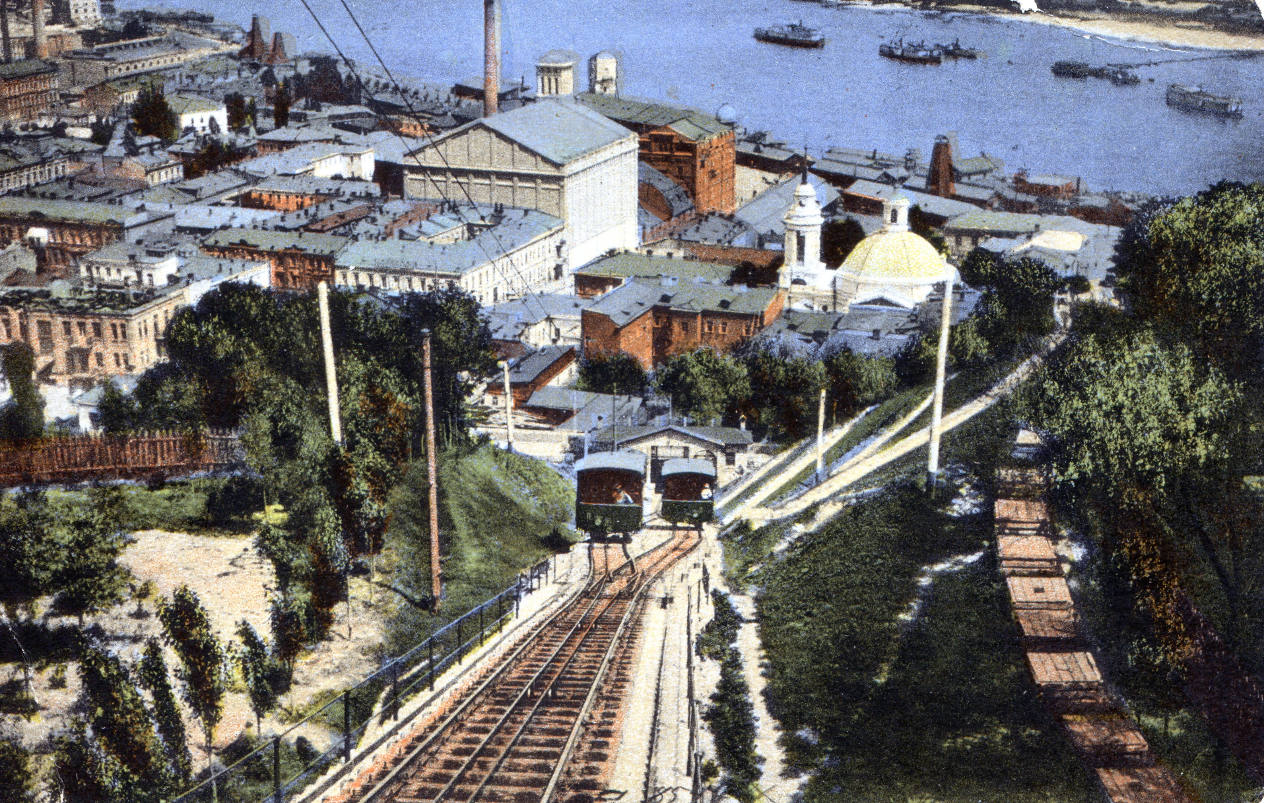
\includegraphics[width=\linewidth]{s-mihpod.jpg}
\end{center}

An old postcard depicting the ravine with the funicular, viewed from the upper station of the funicular. This is, in fact, Borichev Uvoz.


\vspace*{\fill}


\newpage


\vspace*{\fill}

\begin{center}
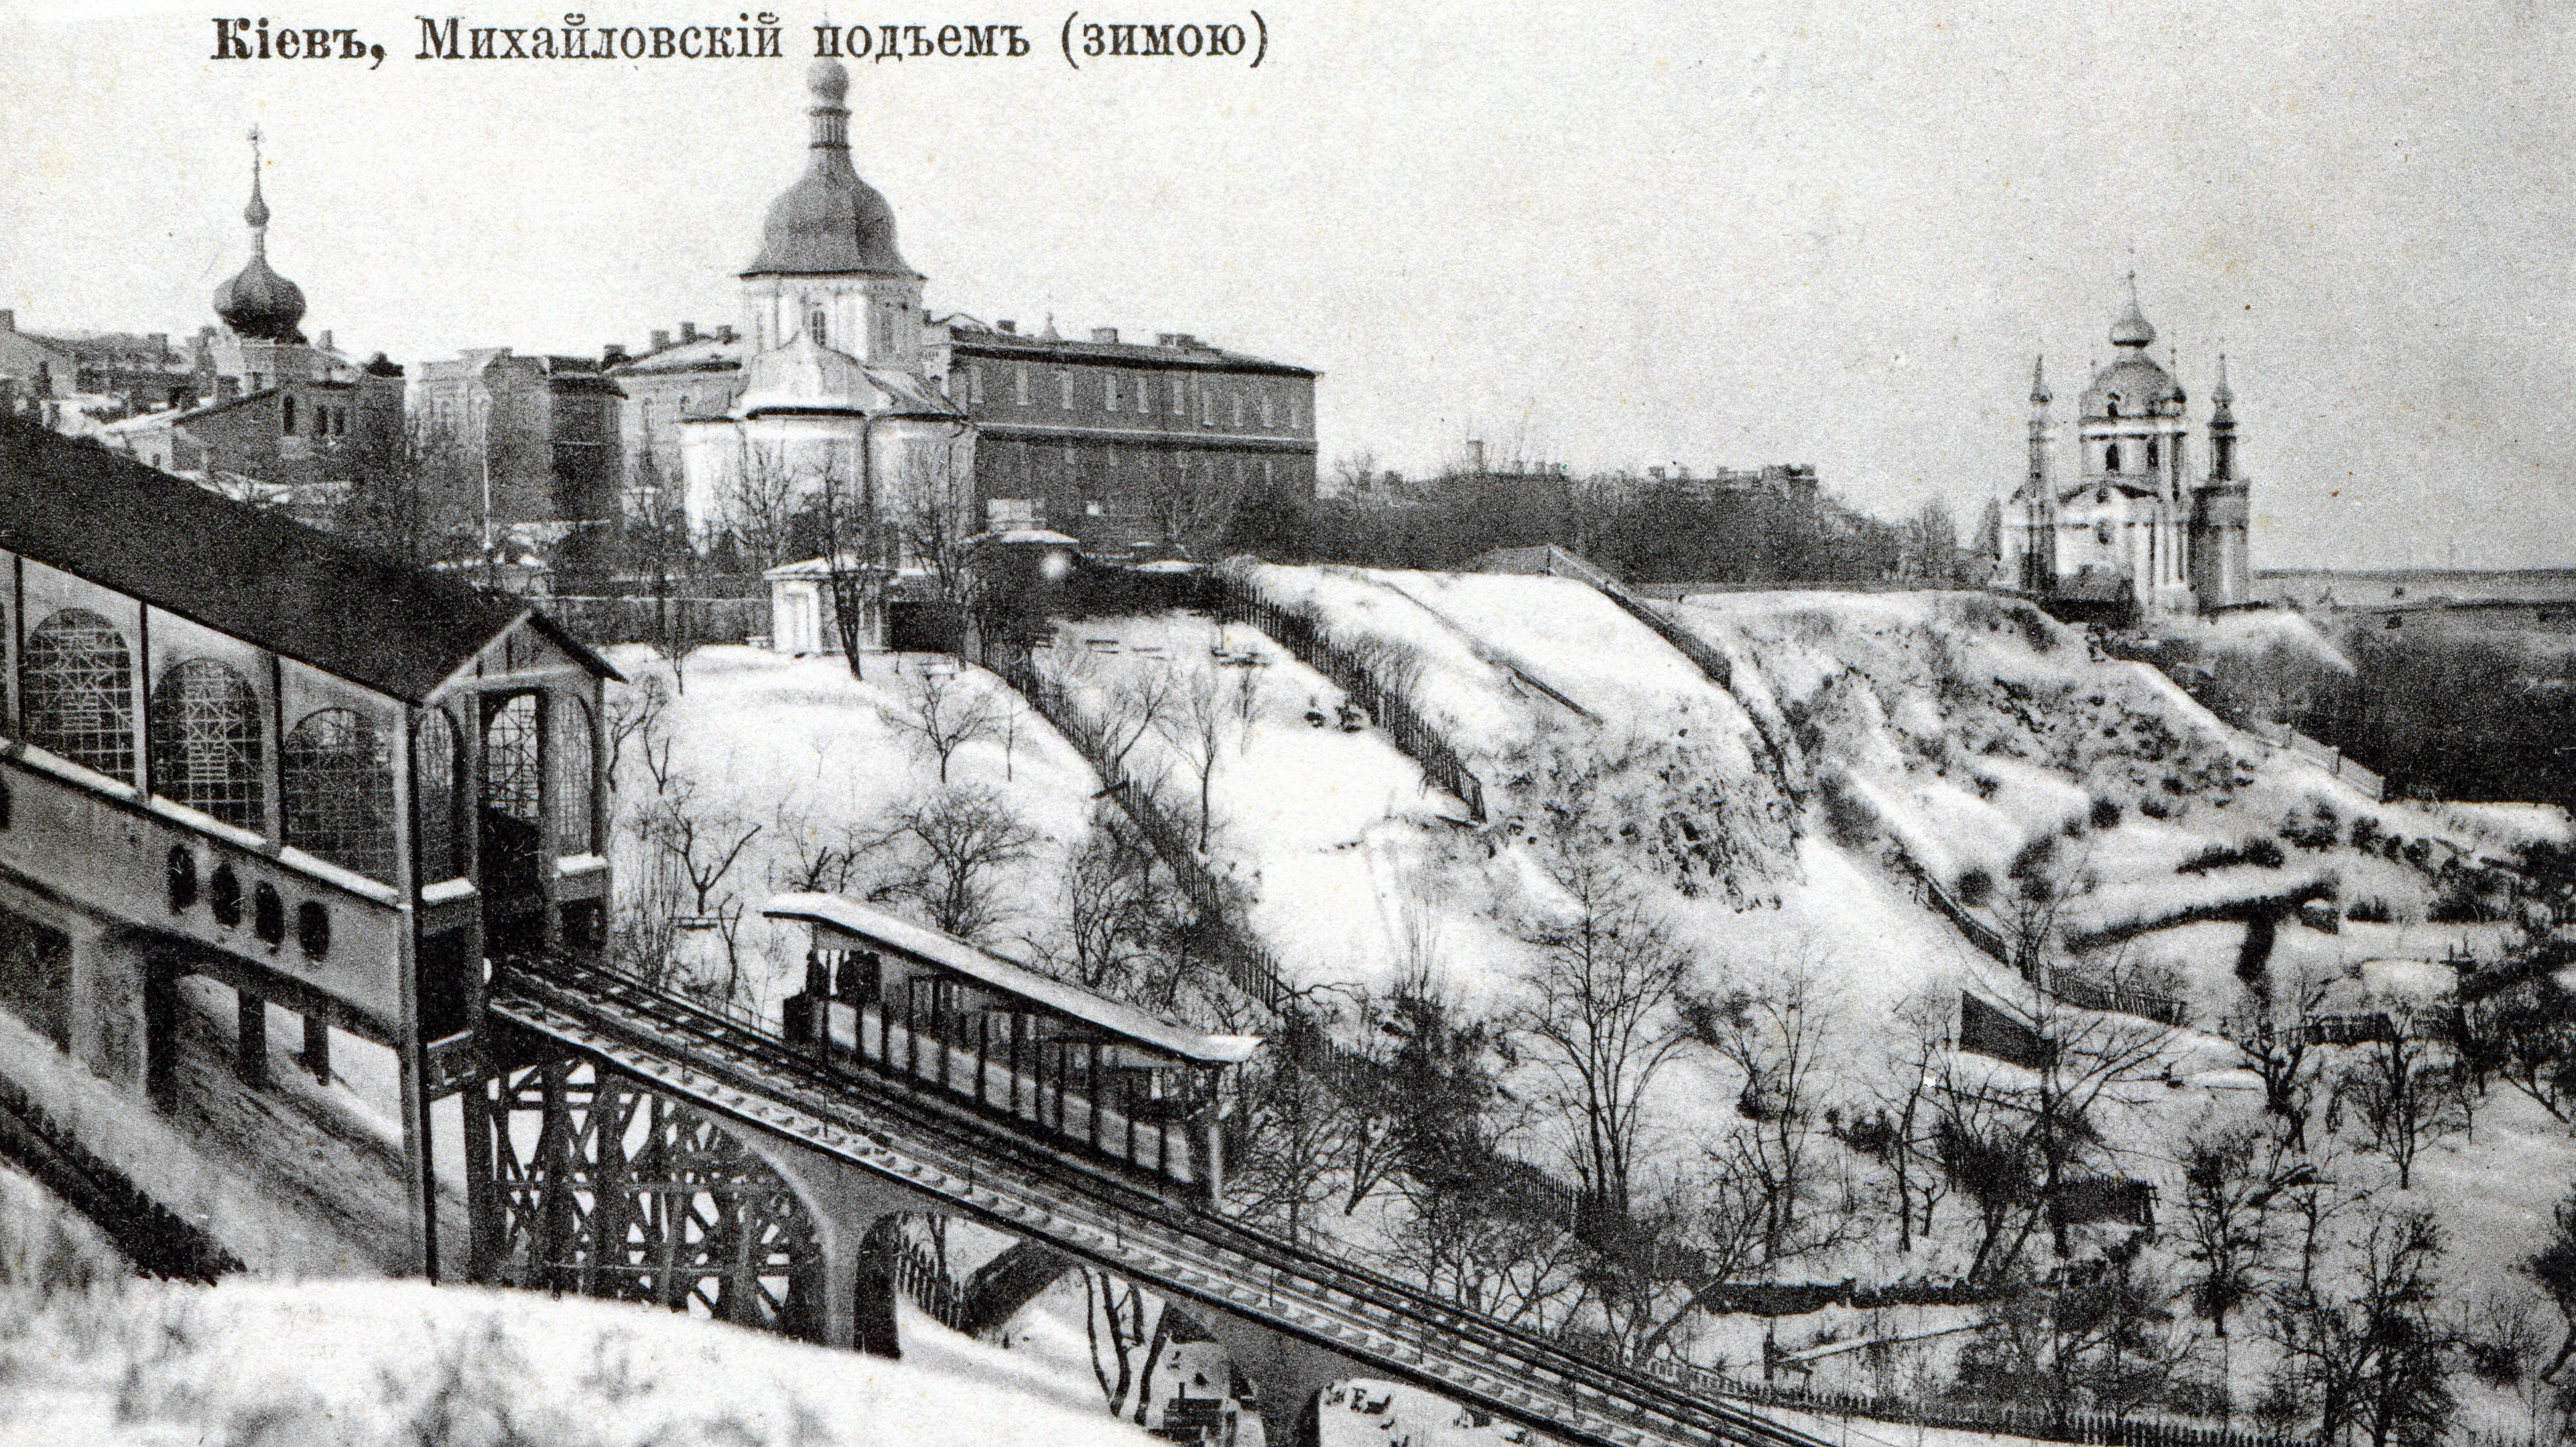
\includegraphics[width=\linewidth]{kuch01.jpg}
\end{center}

Kuchinsky's Garden on an old postcard, when the name Kuchinsky's Garden had already faded from memory and these slopes were referred to as Andreevskaya Gora.

In the foreground is the funicular, which was then called the "Mikhailovsky Ascent." The ravine over which the carriage travels is Borichev Uvoz.

Behind it is the large Church of the Three Holy Hierarchs, possibly on the site of the ancient Vasilievskaya Church, founded by Vladimir the Great.

Behind the church, we can see the building of the Women's Courses, and to the right in the frame is St. Andrew's Church. And the space between it and the funicular, these slopes, are essentially Kuchinsky's Garden.

\vspace*{\fill}

\newpage

\vspace*{\fill}

\begin{center}
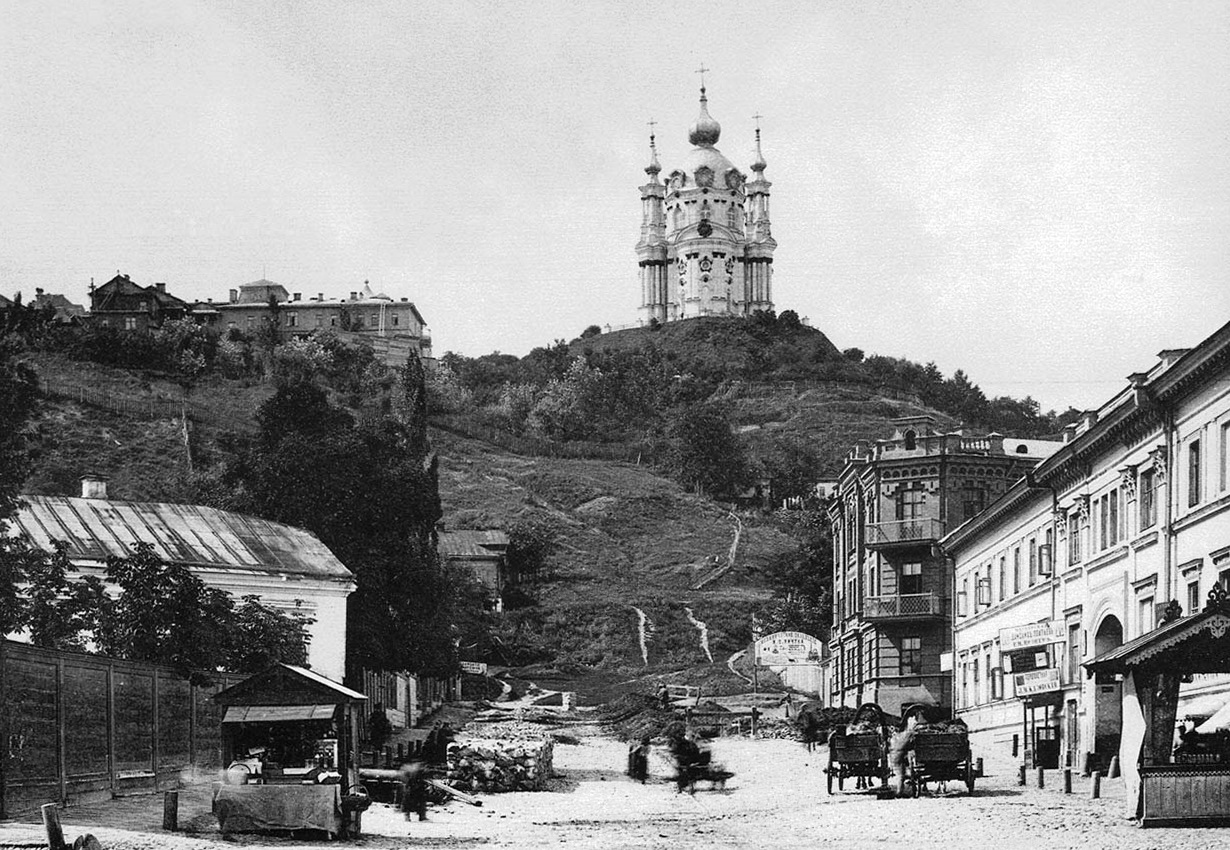
\includegraphics[width=\linewidth]{kuch02.jpg}
\end{center}

A view from a different angle, of St. Andrew's Church, from Andreevskaya Street, which is on Podol district. To the left, we can see the slope of the former Kuchinsky garden.

\vspace*{\fill}

\newpage

\vspace*{\fill}

\begin{center}
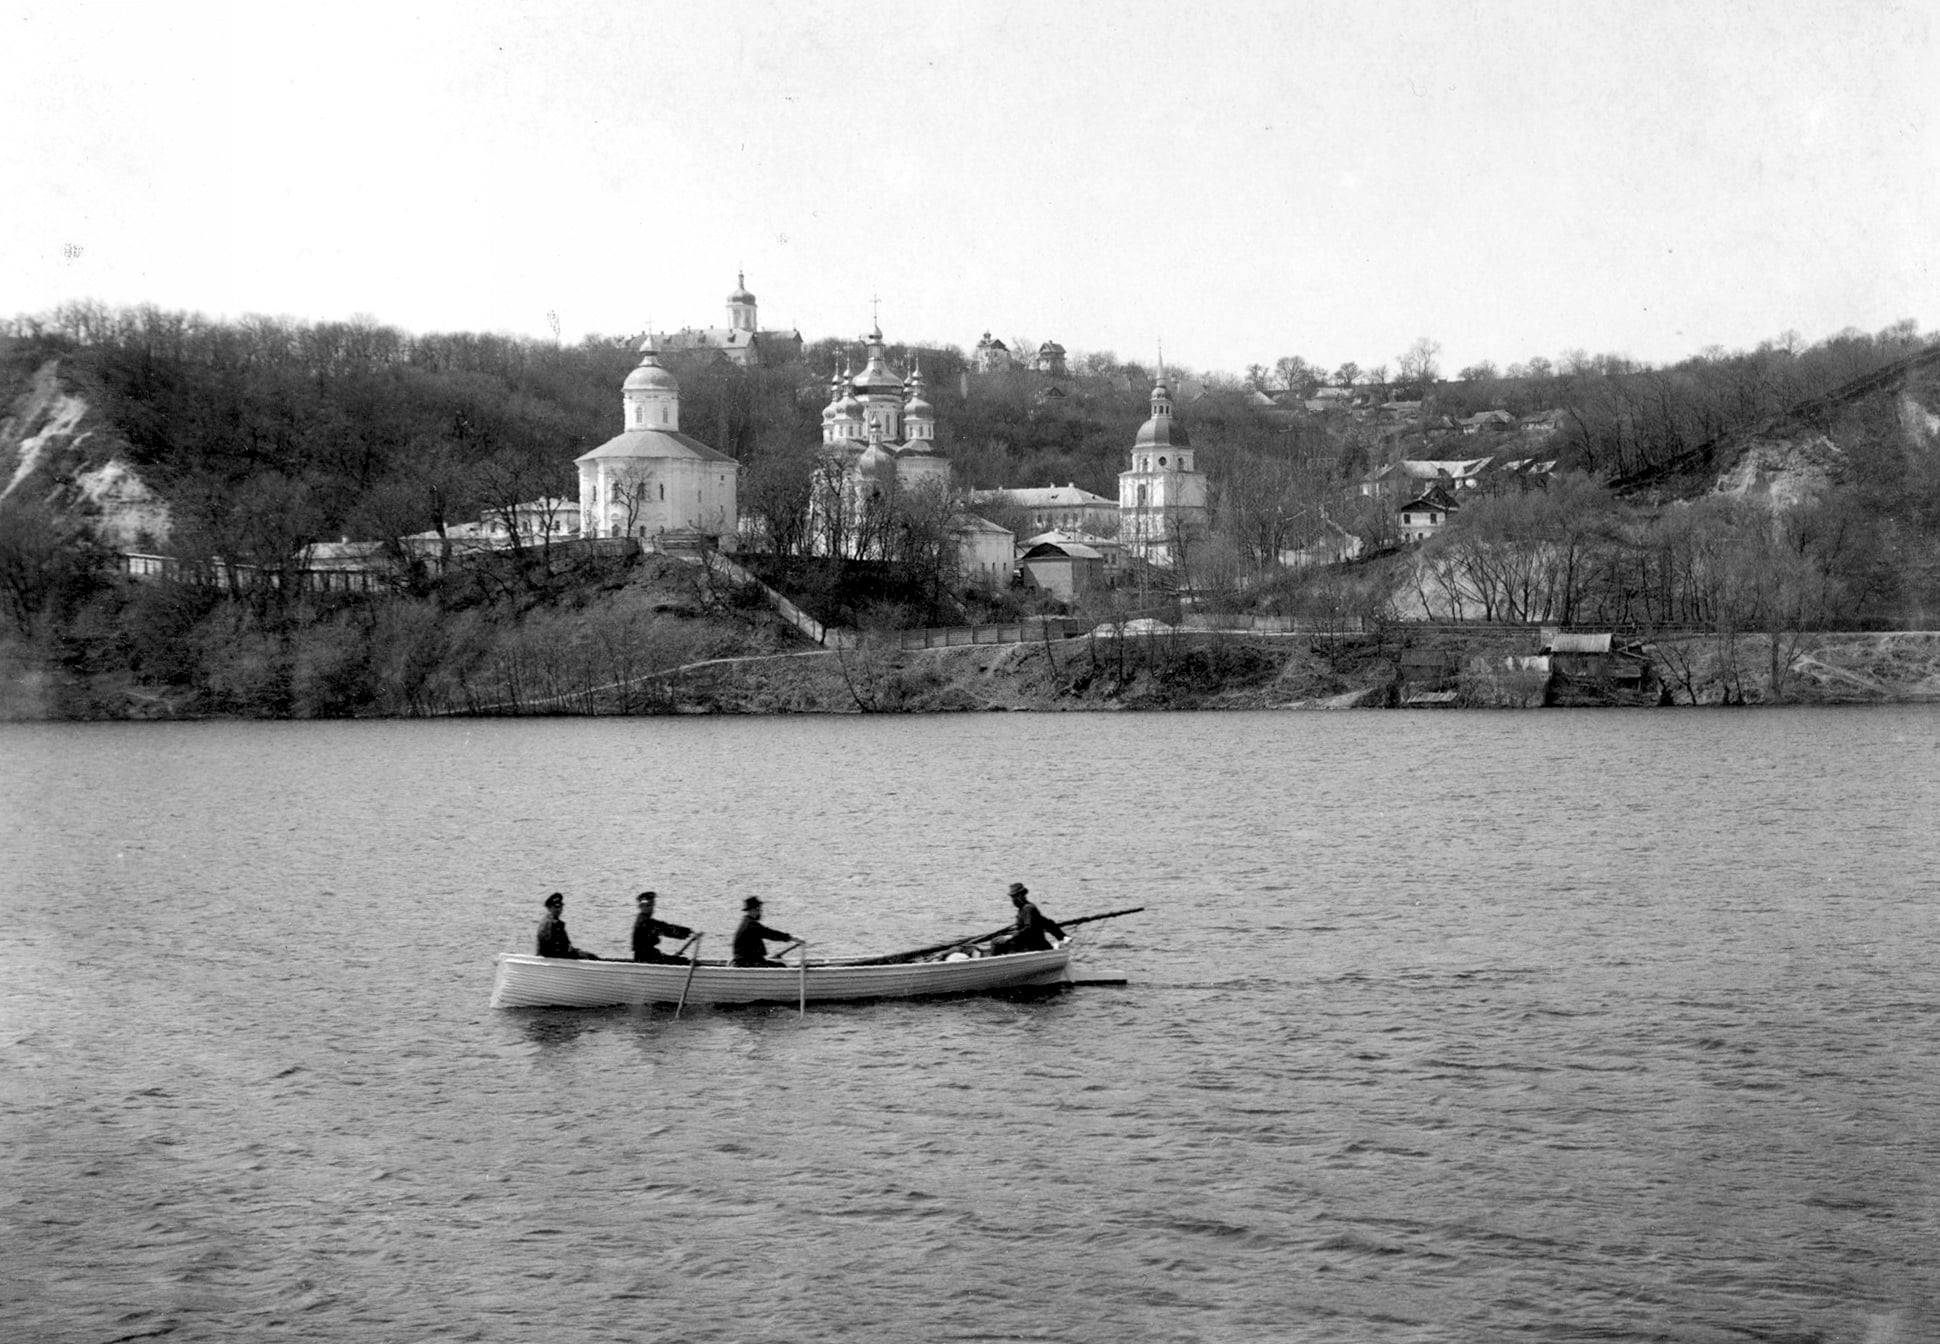
\includegraphics[width=\linewidth]{vyd01.jpg}
\end{center}

View of the Vydubychi area and the monastery. From left to right – the Church of the Miracle of St. Michael in Chonae, the St. George's Cathedral, the Bell Tower with the Church of the Prophet Daniel. At the top of the hill, the buildings of the Ioninsky Holy Trinity Monastery.

\vspace*{\fill}


\newpage

%\backmatter

%\appendix
%\addappheadtotoc


%\input{appendix/dict.tex}

\begin{thebibliography}{999}
\bibitem{zeleninrusalki}
\emph{Избранные труды. Очерки русской мифологии: Умершие неестественною смертью и русалки}. Зеленин Д. К. Индрик, Москва, 1995.

\bibitem{kak}
\emph{Как Владимир идолов низвергал}. Петр Семилетов, DOI 10.5281/zenodo.14212537

\bibitem{volos}
\emph{Скотий бог Волос}. Петр Семилетов, DOI 10.5281/zenodo.14563494
\end{thebibliography}


\end{document} 